\documentclass[11pt]{article}
\usepackage{amsfonts}
\usepackage{amsmath}
\usepackage{booktabs}
\usepackage{caption}
\usepackage[sort,nocompress]{cite}
\usepackage{color}
\usepackage{enumitem}
\usepackage{fancyhdr}
\usepackage{hyperref}
\usepackage{lastpage}
\usepackage{pgfplots}
\usepackage{rotating}
\usepackage{siunitx}
\usepackage{subfigure}
\usepackage{tikz}
\usepackage{tikz-3dplot}
\usepackage{titlesec}
\usepackage{todonotes}
\usepackage{wrapfig}
\usepackage{verbatim}
%\usepackage{showkeys}

\usetikzlibrary{shapes,arrows}

\addtolength{\oddsidemargin}{-0.75in}
\addtolength{\evensidemargin}{-0.75in}
\addtolength{\textwidth}{1.5in}
\addtolength{\topmargin}{-0.75in}
\addtolength{\textheight}{1.5in}
% For 11pt size

\titleformat*{\section}{\large\bfseries}
\titleformat*{\subsection}{\normalsize\bfseries}

\newcommand{\bd}{\partial}
\newcommand{\BL}{\mathrm{BL}}
\newcommand{\bigO}{\mathcal{O}}
\newcommand{\cc}{\mathbf{c}}
\newcommand{\dlp}{{\mathrm{dlp}}}
\newcommand{\ee}{\mathbf{e}}
\newcommand{\ff}{\mathbf{f}}
\newcommand{\FF}{\mathbf{F}}
\renewcommand{\gg}{\mathbf{g}}
\newcommand{\II}{\mathcal{I}}
\newcommand{\mcaption}[2]{\caption{\small \em #1}\label{#2}}
\newcommand{\nn}{\mathbf{n}}
\newcommand{\NN}{{\mathbf{N}}}
\newcommand{\pderiv}[2]{\frac{\partial #1}{\partial #2}}
\newcommand{\pderivtwo}[2]{\frac{\partial^{2} #1}{\partial #2^{2}}}
\newcommand{\pphi}{{\boldsymbol{\phi}}}
\renewcommand{\Re}{{\textrm{Re}}}
\newcommand{\rr}{{\mathbf{r}}}
\newcommand{\RR}{{\mathbb{R}}}
\newcommand{\slp}{{\mathrm{slp}}}
\newcommand{\ssigma}{{\boldsymbol{\sigma}}}
\newcommand{\SLP}{{\mathtt{SLP}}}
\newcommand{\DD}{{\mathcal{D}}}
\renewcommand{\SS}{{\mathcal{S}}}
\newcommand{\ttau}{{\boldsymbol{\tau}}}
\newcommand{\uu}{\mathbf{u}}
\newcommand{\vv}{\mathbf{v}}
\newcommand{\VV}{{\mathcal{V}}}
\newcommand{\xx}{\mathbf{x}}
\newcommand{\yy}{\mathbf{y}}
\newcommand{\thL}{$\theta$--$L$}

\pagestyle{fancy}
\lhead{\footnotesize Bryan Quaife}
\chead{\footnotesize Viscous Erosion of a Porous Medium}
\rhead{\footnotesize \thepage}
\cfoot{}

%\usepgfplotslibrary{external}
%\tikzexternalize



\begin{document}
\begin{center}
Viscous Erosion of a Porous Medium \\
Bryan Quaife, Assistant Professor \\
Florida State University \\
512-436-1148, bquaife@fsu.edu \\
DOE/Office of Science Program Office: ASCR-Applied Mathematics \\
Funding Opportunity Announcement Number: DE-FOA-0001968
\end{center}

%%%%%%%%%%%%%%%%%%%%%%%%%%%%%%%%%%%%%%%%%%%%%%%%%%%%%%%%%%%%%%%%%%%%%%%%%%%%%
\section{Introduction}
Flow-induced erosion deteriorates and reshapes solid material over a
range of scales found in nature, from massive land formations to
centimeter-scale features and patterns. Though less visible, these same
forces are working at the very smallest scales, slowly deteriorating the
individual constituents of porous media (e.g.~soil, sand, or clay) or
biological structures like plaque and biofilms. Motivated by such
examples, we are interested in studying fluid-mechanical erosion in
Stokes flow---the most relevant regime for groundwater and bio-fluid
applications.

\begin{figure}[htp]
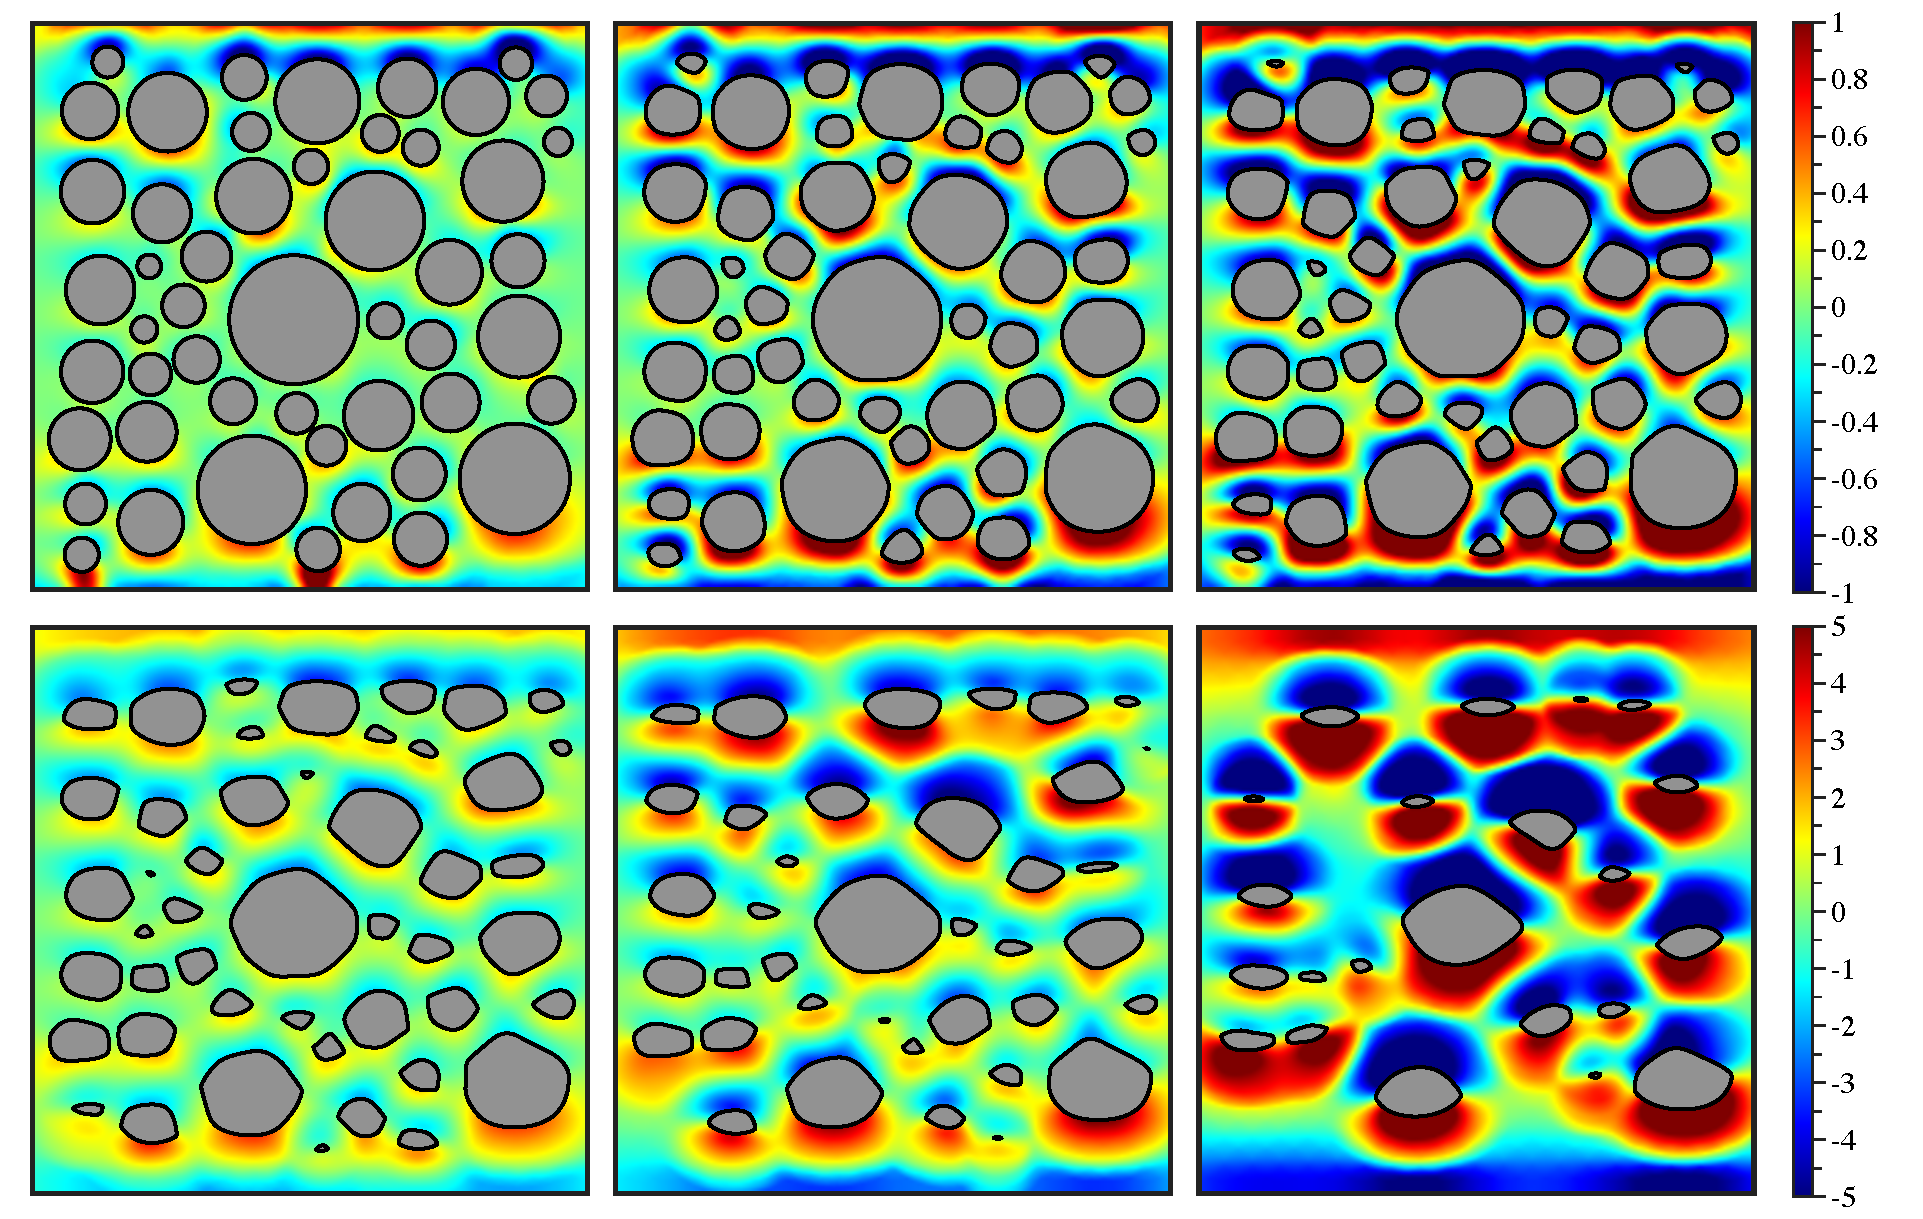
\includegraphics[width=\textwidth]{figs/50bod.pdf}
\caption{\label{fig:50bod} Simulation of 50 bodies eroding in Stokes
flow under the action of fluid-mechanical shear. The flow is horizontal
(left to right) and the 6 snapshots are evenly spaced in time. Color
represents vorticity, which provides a convenient way to visualize local
shear rates. Erosion not only diminishes the size of the bodies but also
alters their shapes considerably. A few well-defined channels develop in
the space between bodies.}
\end{figure}


In our recent publication~\cite{qua-moo2018}, we described a suite of
numerical methods to simulate erosion in a viscous fluid
(Figure~\ref{fig:50bod}).  The highlights of our numerical methods are:
\begin{enumerate}[topsep=0pt,itemsep=-1ex,partopsep=1ex,parsep=1ex]
  \item {\bf Boundary Integral Equation Fluid Solver}: The
  incompressible Stokes equations are solved with a boundary integral
  equation (BIE).  By using a BIE, the complex geometries are naturally
  handled, high-order accurate discretizations are deployed, and fast
  summation methods result in optimal complexity.

  \item {\bf Interface Tracking}: Instead of tracking the $(x,y)$
  coordinates of the boundary of the eroding bodies interface, we track
  the \thL coordinates, where $\theta$ is a local tangent angle, and $L$
  is the total length.  The governing equations of the \thL coordinates
  offers several advantages in the ability to numerically stabilize the
  evolving interface

  \item {\bf Regularizations of the Interface}: Erosion results in
  corners of the bodies at stagnation points of the flow.  We 
  use a regularization term and a smoothing operation to control the
  smoothness of the moving interface.

  \item {\bf Analysis of Single Eroding Bodies}: We validate our method
  by comparing numerical simulations with scaling laws.
\end{enumerate}

\section{Proposed Work}
Having developed and validated numerical methods for simulating viscous
erosion, there are two main directions that our research will follow.
First, additional numerical tools are required to simulate more
realistic scenarios such as bodies that erode and transport, and
extending our work to three dimensions.  Second, we will investigate
physically motivated questions regarding the geometry and flow inside an
eroding porous medium

%%%%%%%%%%%%%%%%%%%%%%%%%%%%%%%%%%%%%%%%%%%%%%%%%%%%%%%%%%%%%%%%%%%%%%%%%%%%%
\subsection{Improved Numerical Methods}
In its current formulation, our bodies are fixed in space.  However, in
reality, eroding bodies are also transported by the flow.  To allow the
bodies to move, there are two additional tools that we will develop.
Bodies get close.


\paragraph{Transport of Bodies:} The PI is experienced with simulating
moving interfaces in Stokes flow.  For example, he has developed
high-order adaptive time stepping methods for simulating deformable
bodies (vesicles) in a viscous fluid~\cite{qua-bir2015b, qua-bir2014,
qua-2016}.   More recently, the PI has graduated a Ph.D.~student that
developed time stepping methods for rigid bodies in a viscous
fluid~\cite{bys-sha-qua2018}.  This work introduces a new time stepping
method

A recent Ph.D.~student from his group

\paragraph{Improved Quadrature:}


%%%%%%%%%%%%%%%%%%%%%%%%%%%%%%%%%%%%%%%%%%%%%%%%%%%%%%%%%%%%%%%%%%%%%%%%%%%%%
\subsection{Physics-Based Understanding of Viscous Erosion}
\todo[inline]{Characterizing anisotropy}
\todo[inline]{Coarse-grained transport (anomalous diffusion}

%%%%%%%%%%%%%%%%%%%%%%%%%%%%%%%%%%%%%%%%%%%%%%%%%%%%%%%%%%%%%%%%%%%%%%%%%%%%%
\section{Biographical Information}
Since 2015, {\bf Bryan Quaife} has been an Assistant Professor in the
Department of Scientific Computing at Florida State University.  He is
also a Research Associate in FSU's Geophysical Fluid Dynamics Institute.
Dr.~Quaife received his Ph.D.~in 2011 in Applied and Computational
Mathematics at Simon Fraser University.  He was a postdoctoral fellow
for four years in Dr.~George Biros' group at the Institute for
Computational Science and Engineering at the University of Texas.  His
research interests include the development of  high-fidelity and
efficient numerical methods for simulating fluid dynamics in complex
geometries.

The co-PI of this project is {\bf Nick Moore}.  Since 2014, Dr.~Moore
has been an Assistant Professor in the Department of Mathematics at
Florida State University.  He is also a Research Associate in FSU's
Geophysical Fluid Dynamics Institute. \todo[inline]{A bit more}


%%%%%%%%%%%%%%%%%%%%%%%%%%%%%%%%%%%%%%%%%%%%%%%%%%%%%%%%%%%%%%%%%%%%%%%%%%%%%
\section{Expected Budget}
\todo[inline]{I can have Michelle put one together.  Funds are needed
for the following}
\begin{itemize}
  \item Summer salary (1 month a year for 3 years)
  \item 2 RA (1 in Math, 1 on DSC)
  \item 1 joint postdoc
  \item Travel
  \item Computers
  \item FSU overhead
\end{itemize}



%%%%%%%%%%%%%%%%%%%%%%%%%%%%%%%%%%%%%%%%%%%%%%%%%%%%%%%%%%%%%%%%%%%%%%%%%%%%%
\bibliographystyle{plain}
\bibliography{refs}

\end{document}
